\section{Κωδικοποίηση \& Αποκωδικοποίηση A-DPCM}

Η μέθοδος DPCM στηρίζεται στο ότι σε ένα σήμα οι διαδοχικές τιμές του θα εμφανίζουμε μεγάλη
συσχέτιση, ενώ το σήμα:
\begin{equation}
  \label{eq:diff_signal}
  d(n) = x(n) - x(n-1)
\end{equation}
\noindent θα εμφανίζει συνήθως μικρότερη συσχέτιση και επιλέγουμε να κωδικοποιήσουμε αυτό αντί του
αρχικού σήματος. Η αντίστροφη διαδικασία γίνεται μέσω της σχέσης:
\begin{equation}
  \label{eq:invert_diff}
  x(n) = d(n) + x(n-1)
\end{equation}
\par Προκειμένου όμως να αποφύγουμε την συσσώρευση σφάλματος λόγω της κβάντισης του σήματος $x(n)$
επιλέγουμε την εξής διαδικασία:
\begin{align}
  &d(n) = x(n) - \hat{x}(n-1) \label{eq:dpcm_dpcm}\\
  &\hat{x}(n) = \hat{d}(n) + \hat{x}(n-1) \label{eq:xhat_dpcm} \\
  &\hat{d}(n) = \bar{Q}[d(n)] \label{eq:diff_quantized}
\end{align}
\noindent όπου με $\bar{Q}[]$ συμβολίζεται ο κβαντιστής.

\par Σε περίπτωση που επιλέξουμε να χρησιμοποιήσουμε περισσότερα από ένα παρελθοντικά δείγματα τότε
οι παραπάνω εξισώσεις γίνονται:
\begin{align}
  &d(n) = x(n) - \sum_{i=1}^m w_i \hat{x}(n-i)  \label{eq:diff_adpcm}\\
  &\hat{x}(n) = \hat{d}(n) + \sum_{i=1}^m w_i \hat{x}(n-i) \label{eq:xhat_adpcm} \\
  &\hat{d}(n) = \bar{Q}[d(n)] \label{eq:diff_quantized_adpcm}
\end{align}

\par Ακόμη, λόγω της διαδικασίας κβάντισης των βαρών για την ενσωμάτωση τους στο header του
συστήματος κωδικοποίησης/αποκωδικοποίησης μπορεί το φίλτρο μας να γίνει ασταθές. Για να το
αποφύγουμε αυτό, αφού εντοπίσουμε τους ασταθείς πόλους μέσω της συνάρτησης \emph{roots} του MATLAB
τους αντικαθιστούμε με πόλους με το αντίστροφο μέτρο. Η διαδικασία αυτή ισοδυναμεί με την εφαρμογή
ενός ολοπερατού φίλτρου στην έξοδο του συστήματος, με μηδενικό στην θέση του ασταθούς πόλου του
φίλτρου πρόβλεψης και κατάλληλα τοποθετημένο πόλο. Η λειτουργία αυτή υλοποιείται μέσω της
συνάρτησης:
\begin{lstlisting}[style=myMatlab]
function [stableWeights] = stabilise_weights(inputWeights)
\end{lstlisting}
\noindent η οποία χρησιμοποιεί τις συναρτήσεις \emph{roots} και \emph{poly} του MATLAB για να
εντοπίσει τους ασταθείς πόλους, δηλαδή αυτούς εκτός του μοναδιαίου κύκλου, και να κατασκευάζει την
κατάλληλη συνάρτηση μεταφοράς ώστε το τελικό σύστημα να είναι ευσταθές.

\noindent
\begin{minipage}{\linewidth}
  \par Το αποτέλεσμα της εκτέλεσης του script που ελέγχει την ορθή λειτουργία της υλοποίησης μας
  φαίνεται στο παρακάτω γράφημα:
  \begin{figure}[H]
    \label{fig:adpcm}
    \centering
    \begin{subfigure}{1.0\textwidth}
      \centering
      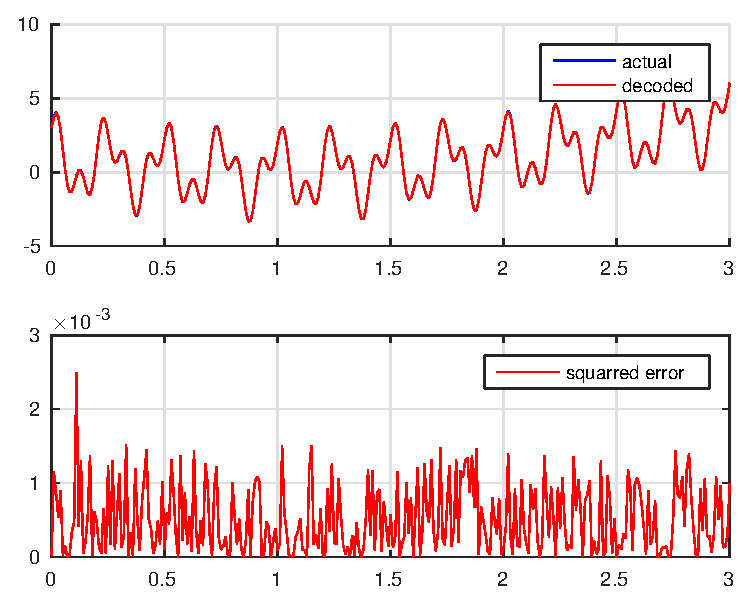
\includegraphics[width=1.0\textwidth]{adpcm.eps}
    \end{subfigure}
    \caption{\protect{Ενδεικτική εφαρμογή A-DPCM}}
  \end{figure}
\end{minipage}


